\documentclass[fleqn]{article}
\oddsidemargin 0.0in
\textwidth 6.0in
\thispagestyle{empty}
\usepackage{import}
\usepackage{amsmath}
\usepackage[backend=bibtex]{biblatex}
\usepackage[utf8]{inputenc}
\usepackage{csquotes}
\usepackage{graphicx}
\usepackage{flexisym}
\usepackage{calligra}
\usepackage{amssymb}
\usepackage{bigints} 
\usepackage[english]{babel}
\usepackage{float}
\usepackage[colorinlistoftodos]{todonotes}
\usepackage{blindtext}
\usepackage{hyperref}

\addbibresource{references.bib}

\hypersetup{
  colorlinks=true,
  linkcolor=blue,
  filecolor=magenta,      
  urlcolor=cyan,
  pdfpagemode=FullScreen
}

\DeclareMathAlphabet{\mathcalligra}{T1}{calligra}{m}{n}
\DeclareFontShape{T1}{calligra}{m}{n}{<->s*[2.2]callig15}{}
\newcommand{\scriptr}{\mathcalligra{r}\,}
\newcommand{\boldscriptr}{\pmb{\mathcalligra{r}}\,}


\setlength{\arrayrulewidth}{0.5mm}
\setlength{\tabcolsep}{18pt}
\renewcommand{\arraystretch}{1.5}

\definecolor{hwColor}{HTML}{AD53BA}

\begin{document}

  \begin{titlepage}

    \newcommand{\HRule}{\rule{\linewidth}{0.5mm}}

    \center

    \begin{center}
      
\includegraphics[height=11cm, width=11cm]{asu.png}
    \end{center}

    \vline

    \textsc{\LARGE Advanced Laboratory I}\\[1.5cm]

    \HRule \\[0.5cm]
    { \huge \bfseries Pulsed NMR}\\[0.4cm] 
    \HRule \\[1.0cm]

    \textbf{Behnam Amiri}

    \bigbreak

    \textbf{Prof: Ralph Chamberlin}

    \bigbreak

    \textbf{Lab Partners: Daniel Henningsen, Micah Smith, Srihari Ravi}

    \bigbreak

    \textbf{{\large \today}\\[2cm]}

    \vfill

  \end{titlepage}

  \textbf{Abstract}

  \vspace{10px}

  This lab report represents the experimental procedure we did to learn about the \emph{Pulsed Nuclear 
  Magnetic Resonance (Pulsed NMR)}. The Nuclei is studied in the presence of a magnetic field.

  \vspace{20px}


  \textbf{I. Introduction}

  \vspace{10px}

  Nuclear magnetic resonance (NMR) was worked on in 1945 by 2 physicists, Edward M. Purcell and Felix Bloch. They were given
  the 1952 Noblem Prize in physics for their work. \textcite{One} Basically NMR is about the spins of protons when a magnetic field 
  is applied and how the magnetic fields can line up protons.

  \vspace{20px}


  \textbf{II. Background Information}

  \vspace{10px}

  The discovery of NMR goes back to the 1930s when Isidor Isaac Rabi and his team were measuring the the magnetic properties of 
  nuclei like hydrogen. They observed how an oscillating magnetic field is able to effect principal magnetic orientation 
  of nuclei.\textcite{Two}

  \vspace{20px}


  \textbf{III. Theory}

  \vspace{10px}

  The precession rate (resonance frequency) of protons depends linearly on the magnetic field and can be calculated using the following equation
  $$
    f_0(MHz)=4.258 ~ B_0
  $$
  In order to calculate the spin-spin relaxation time, we could use the below equation.
  $$
    M=M_0 ~ exp \left(-\dfrac{t}{T}\right)
  $$


  \textbf{IV. Experimental Procedure}

  \vspace{10px}

  For this experimental, we followed the steps provived in the lab instruction. \textcite{Three}
  
  \vspace{20px}

  \textbf{V. Results}

  \vspace{10px}

  The following plots are our results from this Pulsed NMR experiment. The second and third plots data are from Dr.Chamberlin due to the fact that our recorded data 
  was not correct for some reason.

  \pagebreak

  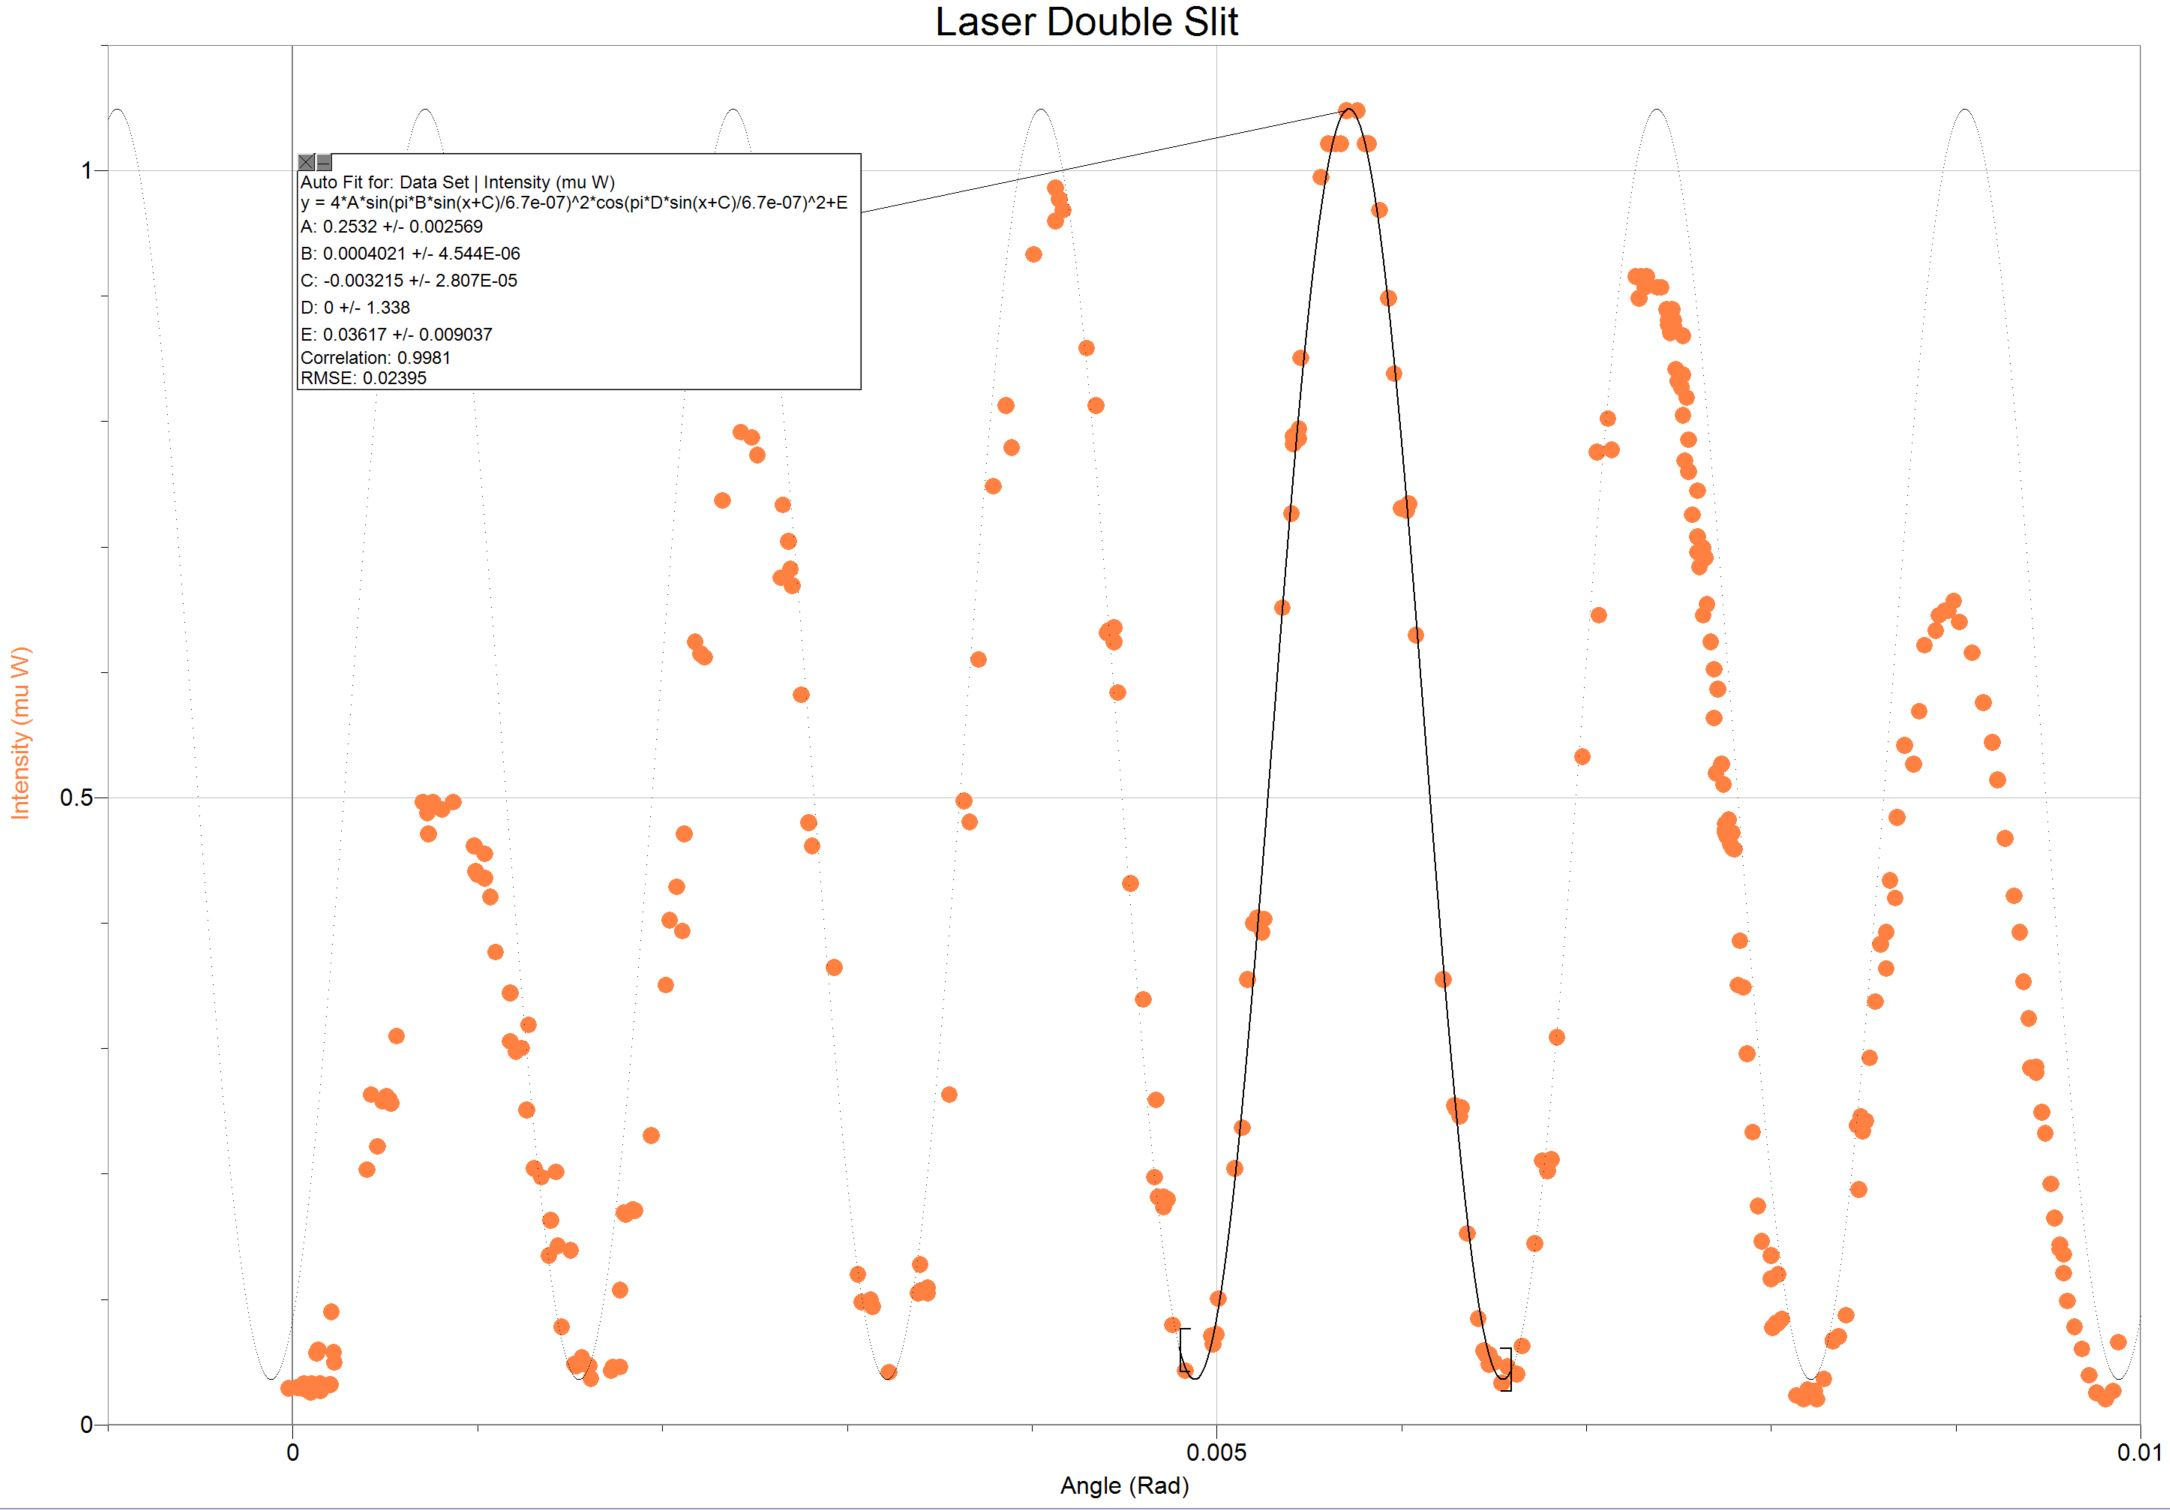
\includegraphics[height=9cm, width=14cm]{Fig1.JPG}
  
  \textbf{Figure 1, Apparent Spin-Spin Relaxation Time $(T_2^*)$}

  \vspace{10px}

  In this plot, the amplitudes is represented as a function of time. We adjust the oscilloscope to see 
  the full FID on it clearly and recorded the amplitudes as a function of time for 9 values using the cursor on the 
  screen. My experimental value of $T_2^*$, and its uncertainty is $63.21 \pm 4.254 ~ \mu s$ which is a smaller than $0.1 ~ ms$ as 
  it was mentioned on the lab instructions. Also, I could use a \textbf{Curve Fit} to the amplitudes to find a experimentally value for $T_2^*$.
  The magnetic field can be found with the help of $f_0=4.258 B_0$. We set the frequency to $15.18805 ~ MHz$, 
  therefore $B_0=3.5669 ~ KG$. Essentially, an electromagnetic signal lines up the spin of protons with the magnetic field in the XY plane.
  When the component is in the XY plane, then the precessing magnetisation will induce 
  a corresponding voltage which oscillates and converges at the end. the maximum amplitude happens when at $90^{\circ}$.
  It's only an apparent relaxation time since the direction that it is coming is from the differences in precession frequency, and not 
  from the changes in the precession frequency due to changes in the local magnetic field.

  \begin{center}
    \begin{tabular}{ |c| } 
     \hline
     $M=M_0 ~ exp \left(-\dfrac{t}{T_2^*}\right)$  \\ 
     $M_0=4202 \pm 378.0 ~ mV$ \\ 
     $T_2^*=63.21 \pm 4.254 ~ \mu s$ \\
     \hline
    \end{tabular}
  \end{center}
        
  \pagebreak

  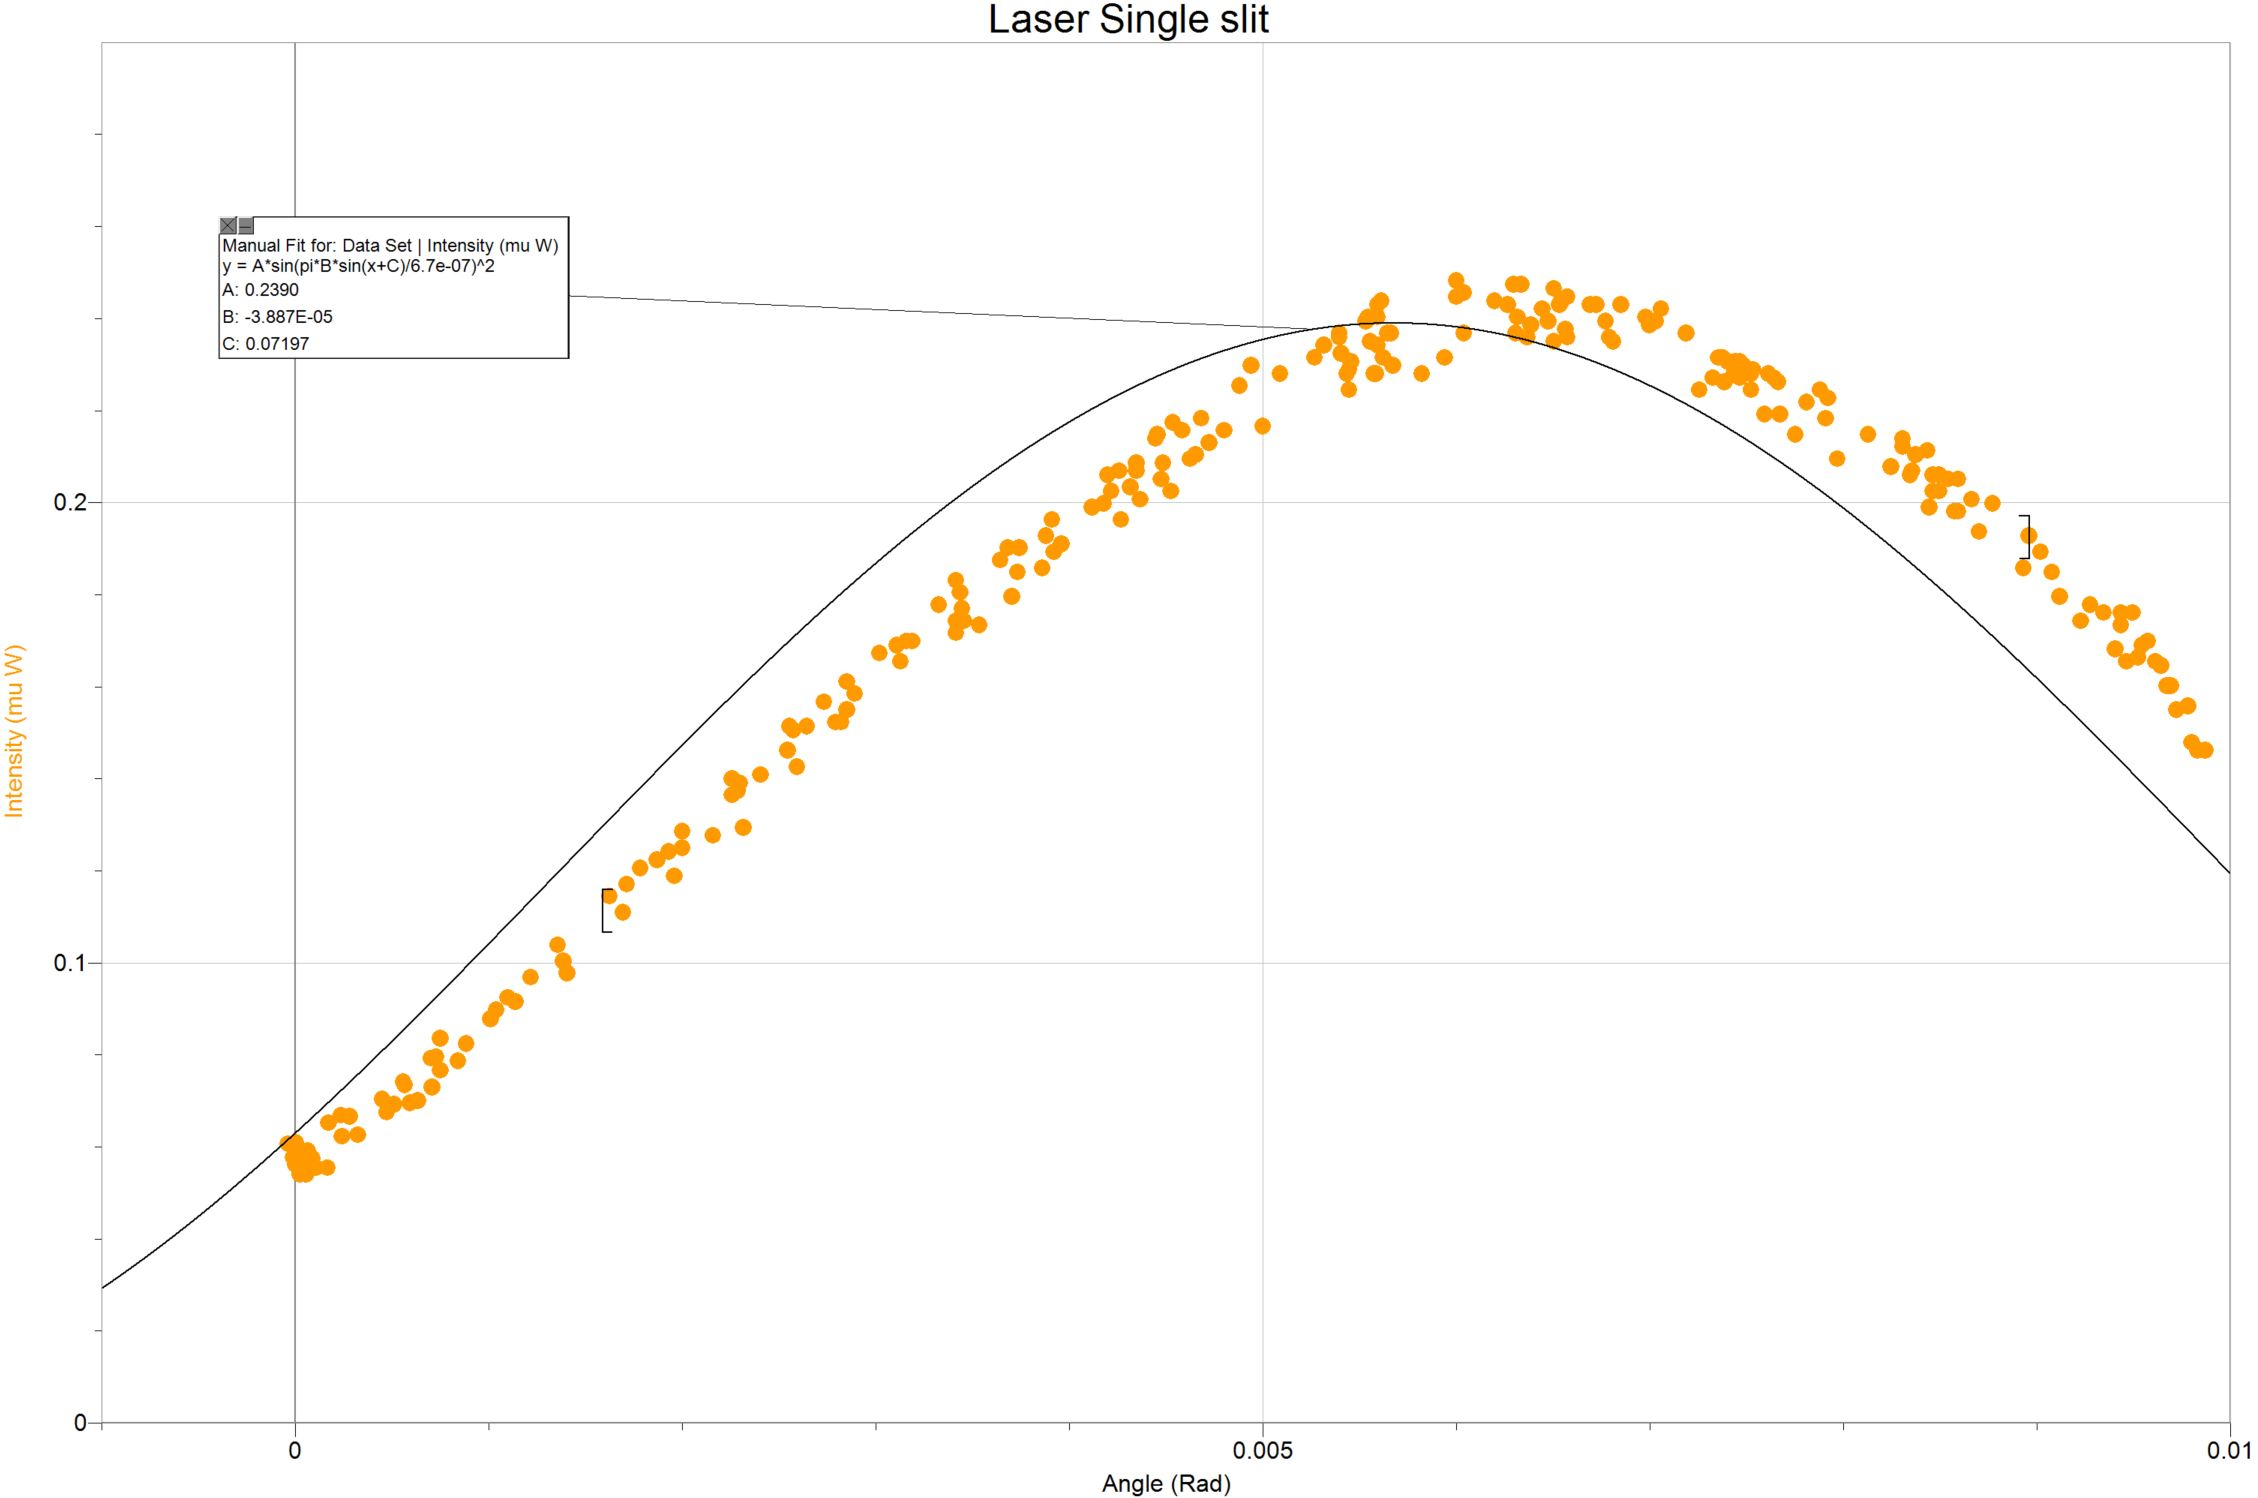
\includegraphics[height=9cm, width=14cm]{Fig2.JPG}

  \textbf{Figure 2, Spin-Lattice Relaxation Time $(T_1)$}

  \vspace{10px}

  This is the plot of the amplitude of the magnetization immediately following the B-pulse as a function of delay time. 
  I used a quadratic function to fit the data. It was found the value of $T_{min}$ as $18.88 ~ ms$ and my best 
  experimental value for $T_1$ and its uncertainty, deduced from the fit parameters for the quadratic is
  $27.2380 \pm 0.01401 ~ ms$. 
  We measured the variable \textbf{Repetition Time} by changing time scale until we saw two pulses. The time between the 
  two pusles was $7.6 \times 2= ~ 15.2 ~ ms$ which is the approximate spin-lattice relaxation time $T_1^'$. The 
  approximate spin-lattice relaxation time is consistent with my value since they are on around the same range of magnitudes.

  \begin{center}
    \begin{tabular}{ |c| } 
     \hline
     Avg A = $A(t-a)^2+B$  \\ 
     A: $25.65 +/- 0.6769 ~ mV/ms^2$ \\
     a: $18.88 +/- 0.01401 ms$ \\ 
     B: $19.27 +/- 1.270 ~ mV$  \\ 
     Correlation: $0.9927$ and RMSE: 4.131 \\
     \hline
    \end{tabular}
  \end{center}

  \pagebreak

  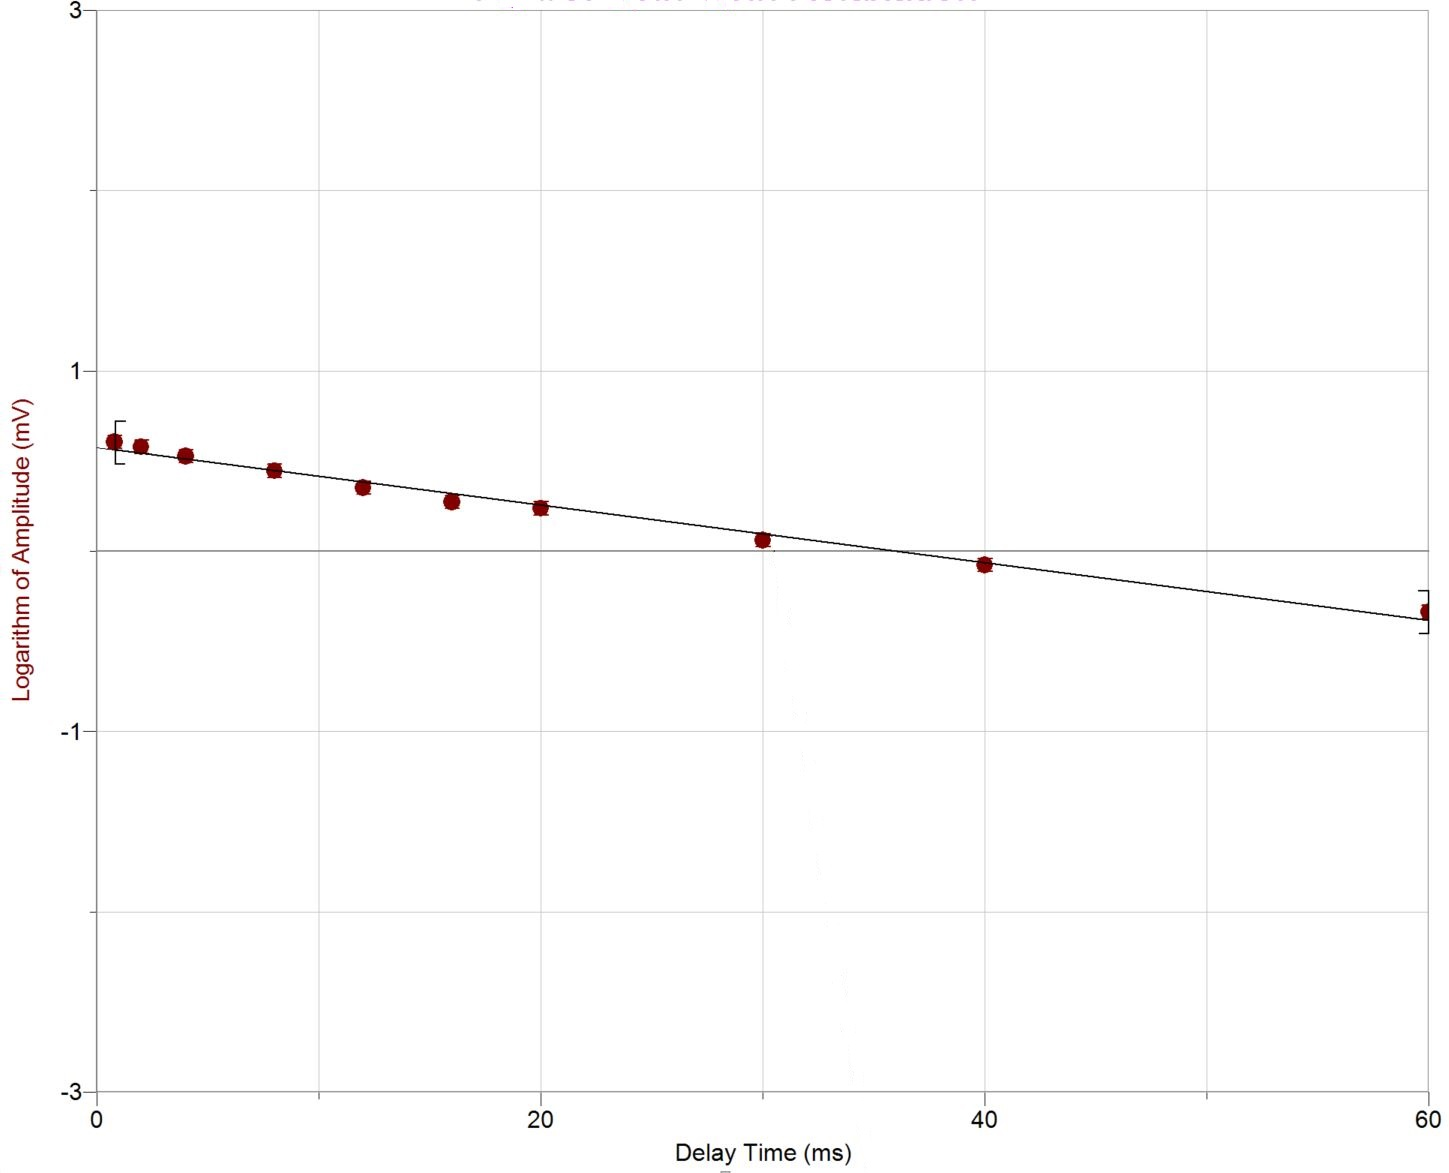
\includegraphics[height=9cm, width=14cm]{Fig3.JPG}

  \textbf{Figure 3, Spin-Spin Relaxation Time $(T2)$}

  \vspace{10px}

  This plot is for the echo amplitude as a function of the total \textbf{Delay Time} $(2 \tau)$. The vertical axis is 
  the logarithm of amplitudes. I used a simple exponential function to fit my data on a Semi-Logarithmic graph. My best experimental value for $T_2$, and its uncertainty, deduced from the
  exponential fit parameters is $22.82 \pm 1.082 ~ ms$. 
  
  We know that the spin-spin relaxation time concerns changes in their precession frequency. In other words, it is the time that spins stop precessing
  synchronously. There is a difference between the apparent spin-spin relaxation time and  spin-spin relaxation time. the apparent one is 
  differences in spins precession frequency that causes spins' dealy time but spin-spin relaxation one is about changes in precession frequency 
  due to changes in the local magnetic field. From the lab document we learned "\emph{The analogy involves changes in
  the local gravity (or vertical acceleration) that would change the precession frequency of the top.}" Hence, the two values are different.

  \begin{center}
    \begin{tabular}{ |c| } 
     \hline
     $M=M_0 ~ exp \left(-\dfrac{t}{T_2^*}\right)$  \\ 
     $M_0=4.054 \pm 0.08151 ~ mV$ \\ 
     $T_2^*=22.82 \pm 1.081 ~  ms$ \\
     \hline
    \end{tabular}
  \end{center}

  \pagebreak


  \textbf{VI. Discussion}

  \vspace{10px}

  By following the lab report document for this experiment, we were able to find the relaxation time values. 
  
  \vspace{20px}


  \textbf{VII. Conclusions}

  \vspace{10px}

  In this experiment, Pulsed Nuclear Magnetic Resonance, we were able to calculate spin-latticeand spin-spin relaxation times. The spins start
  to precess about the Z axis ($\hat{k}$). Right after the spins are in the XY plane, and the precessing start to happen, part of the spins move 
  slower in comparesion to other spins which causes some differences between them. 
  After the Initial $90^{\circ}$ pulse, the protons spins are aligned in XY plane. They start to spread out and then once we hit them with $180^{\circ}$ 
  pulse then the spins are pointed in the opposite directions and instead of spreading out they get togother. 

  
  \vspace{20px}


  \printbibliography

\end{document}
